\subsection{PROPERTIES OF GRADED COGEBRAS OF TYPE N}

PROPOSITION 5. (i) Let E be a graded cogebra admitting a counit \(\gamma\) ; then \(\gamma\) is a homogeneous linear form of degree 0.

\begin{enumerate}
\def\labelenumi{(\roman{enumi})}
\setcounter{enumi}{1}
\tightlist
\item
  Suppose further that there exists an element \(e \in \mathbf{E}\) such that \(\mathbf{E}_0 = \mathbf{A}e\) and \(\gamma(e) = 1\) . Then the kernel \(\mathbf{E}_{\gamma}\) of \(\gamma\) is equal to \(\mathbf{E}_{+} = \sum_{n \geqslant 1} \mathbf{E}_n, c(e) = e \otimes e\) and
\end{enumerate}

\[
c (x) \equiv x \otimes e + e \otimes x (\mathrm{mod.} \mathrm{E} _ {+} \otimes \mathrm{E} _ {+})\tag{19}
\]

for all \(x \in \mathbf{E}_{+}\) .

\begin{enumerate}
\def\labelenumi{(\roman{enumi})}
\tightlist
\item
  It suffices to verify that \(\gamma(x) = 0\) for \(x \in \mathbf{E}_n\) , for all \(n \geqslant 1\) . Since \(c\) is a graded homomorphism of degree 0,
\end{enumerate}

\[
c (x) = \sum_ {0 \leqslant j \leqslant n} \left(\sum_ {i} y _ {i j} \otimes z _ {i, n - j}\right)\tag{20}
\]

with, for all \(j\) such that \(0 \leqslant j \leqslant n\) , \(y_{ij}\) and \(z_{ij}\) in \(\mathbf{E}_j\) ; applying (16) (no. 2) we obtain

\[
x = \sum_ {0 \leqslant j \leqslant n} \left(\sum_ {i} \gamma (y _ {i j}) z _ {i, n - j}\right) = \sum_ {0 \leqslant j \leqslant n} \left(\sum_ {i} \gamma (z _ {i, n - j}) y _ {i j}\right),
\]

whence, equating the components of degree 0 and degree n on the two sides

\[
x = \sum_ {i} \gamma (y _ {i 0}) z _ {i n} = \sum_ {i} \gamma (z _ {i 0}) y _ {i n}
\]

\[
0 = \sum_ {i} \gamma (y _ {i n}) z _ {i 0} = \sum_ {i} \gamma (z _ {i n}) y _ {i 0}
\]

and therefore \(\gamma(x) = \sum_{i} \gamma(y_{in})\gamma(z_{i0}) = \gamma(0) = 0\) .

\begin{enumerate}
\def\labelenumi{(\roman{enumi})}
\setcounter{enumi}{1}
\tightlist
\item
  Since \(\operatorname{Ker}(\gamma)\) and \(\mathbf{E}_{+}\) are both supplementary sub-A-modules of \(Ae = E_0\) and \(\mathbf{E}_{+} \subset \operatorname{Ker}(\gamma)\) by (i), \(\mathbf{E}_{+} = \operatorname{Ker}(\gamma)\) (II, § 1, no. 8, Remark 1); the other assertions follow from Proposition 4 of no. 2.
\end{enumerate}

PROPOSITION 6. Let E be a graded cogebra over A. In order that, for every commutative A-algebra B, with the trivial graduation, the graded A-algebra of type Z Homgr \(_{A}\) (E, B) (no. 2) be anticommutative (§ 4, no. 9, Definition 7), it is necessary and sufficient that, if \(\sigma_{g}\) denotes the automorphism of the A-module E \(\otimes_{A} E\) such that

\[
\sigma_ {g} (x _ {p} \otimes x _ {q}) = (- 1) ^ {p q} x _ {q} \otimes x _ {p}
\]

for \(x_{p} \in \mathbf{E}_{p}, x_{q} \in \mathbf{E}_{q}\) , where \(p\) and \(q\) are arbitrary elements of \(\mathbf{N}\) , the diagram

\begin{enumerate}
\def\labelenumi{(\arabic{enumi})}
\setcounter{enumi}{20}
\tightlist
\item
\end{enumerate}

\pandocbounded{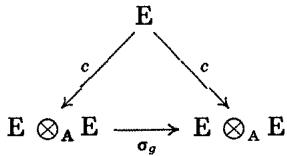
\includegraphics[keepaspectratio]{images/part004_b841500b.jpg}}

be commutative.

The proof is analogous to that of Proposition 2 of no. 2.

When the graded cogebra E satisfies the condition of Proposition 6, it is said to be anticocommutative.

Example. It follows immediately from formula (8) of no. 1 that for every A-module M, the graded cogebra \(\bigwedge(M)\) is anticocommutative.

